\section{Double-counting the evidence}

\begin{enumerate}
\item we need 5 parameters

\item 
\begin{table}[H]
\centering
\caption{Values for Y=T}
\label{Probabilities}
\begin{tabular}{|l|l|l|}
\hline
\textbf{X1} & \textbf{X2} & \textbf{Y=T}  \\ \hline
T           & T           & 0.8*0.5 = 0.4 \\ \hline
T           & F           & 0.8*0.5=0.4   \\ \hline
F           & T           & 0.2*0.5 = 0.1 \\ \hline
F           & F           & 0.2*0.5 = 0.1 \\ \hline
\end{tabular}
\end{table}
\begin{table}[H]
\centering
\caption{Values for Y=F}
\label{Probabilities}
\begin{tabular}{|l|l|l|}
\hline
\textbf{X1} & \textbf{X2} & \textbf{Y=F}   \\ \hline
T           & T           & 0.3*0.1 = 0.03 \\ \hline
T           & F           & 0.3*0.9 = 0.27 \\ \hline
F           & T           & 0.7*0.1 = 0.07 \\ \hline
F           & F           & 0.2*0.5 = 0.1  \\ \hline
\end{tabular}
\end{table}
\begin{table}[H]
\centering
\caption{Prediction}
\label{my-label}
\begin{tabular}{|l|l|l|}
\hline
\textbf{X1} & \textbf{X2} & \textbf{Y Prediction} \\ \hline
T           & T           & T                     \\ \hline
T           & F           & T                     \\ \hline
F           & T           & T                     \\ \hline
F           & F           & F        \\ \hline
\end{tabular}
\end{table}

\item For the Naive Bayes decision function $f(X_1, X_2)$,
  the error rate is:
  \begin{equation*}
    \sum_{X_1,X_2,Y} \ind{Y \ne f(X_1,X_2)}P(X_1, X_2, Y).
  \end{equation*}
  For this question, we will assume that the true data distribution is
  exactly the same as the Naive Bayes distribution, so we can write
  $P(X_1, X_2, Y)$ as $P(Y)P(X_1 \mid Y)P(X_2 \mid Y)$.

  \begin{enumerate}
    \item When using both attirbutes we need to add error when Y=T and when Y=F \\
Using table 3 above \\
For Y = T we have error when $X_1 =F\; and \; X_2 = F$\\
For Y = F we have error in the other 3 cases \\
Adding the errors based on the formula above \\
$= 0.1 * 0.5 + 0.03*0.5+0.27*0.5 + 0.07*0.5 = 0.235$


    \item When using only $X_1$ we will get error when $X_1 = T when Y = F and X_1 = F when Y = T $\\
	error = $0.3*0.5+0.2*0.5$ \\
		= 0.250
   
    \item Similarly for $X_2$ we can computer error \\
	error = $0.5*0.5 + 0.1*0.5$ \\
		= 0.300

    \item  Error rate decreases 
            
  \end{enumerate}

\item Now, suppose that we create a new attribute $X_3$,
  which is an exact copy of $X_2$. So, for every training example,
  attributes $X_2$ and $X_3$ have the same value, $X_2 = X_3$.

  \begin{enumerate}
  \item No they are co-related

  \item
\begin{table}[H]
\centering
\caption{Prediction for Y}
\label{my-label}
\begin{tabular}{llllll}
X1 & X2 & X3 & Y=T   & Y=F   & Y Pred \\
T  & T  & T  & 0.2   & 0.003 & T      \\
T  & F  & T  &       &       &        \\
T  & F  & F  & 0.2   & 0.243 & F      \\
T  & T  & F  &       &       &        \\
F  & T  & F  &       &       &        \\
F  & T  & T  & 0.050 & 0.007 & T      \\
F  & F  & F  & 0.050 & 0.567 & F      \\
F  & F  & T  &       &       &       
\end{tabular}
\end{table}
 As in 3.3 above calculating the error based on true probabilities mentioned in table 1 and 2.
	error = 0.3
    
  \end{enumerate}

\item Naive Bayes assumes conditional independence but $X_2$ and $X_3$ are co-related


\item No because logistic regression assumes no such conditions and will not choose either $X_2$ or $X_3$

\item :

  \begin{enumerate}
    \item Using the Bayes decision rule and as given $X_2$ and $X_3$ are equal. Substituting these values and since we want to choose $P(Y = T | X_i)$ , the decision should be greater than or equal to 1 \\
	\begin{align*}
		\dfrac{ p * q * q}{(1-p) (1-q) (1-q)} \ge 1 \\
		pq^2 \ge (1-p) (1-q)^2 \\
		pq^2 \ge (1-q)^2 - p(1-q)^2 \\
		p(q^2 + (1-q)^2) \ge (1-q)^2 \\
		p \ge \dfrac{(1-q)^2}{(q^2 + (1-q)^2)}
	\end{align*}



    \item Similar to part above using True rule 
	\begin{align*}
	\dfrac{ p * q }{(1-p) (1-q)} \ge 1 \\
	pq \ge (1-p) (1-q) \\
	p \ge (1-q)\\
	\end{align*}


    \item 	
	\begin{figure}[ht!]
	\centering
	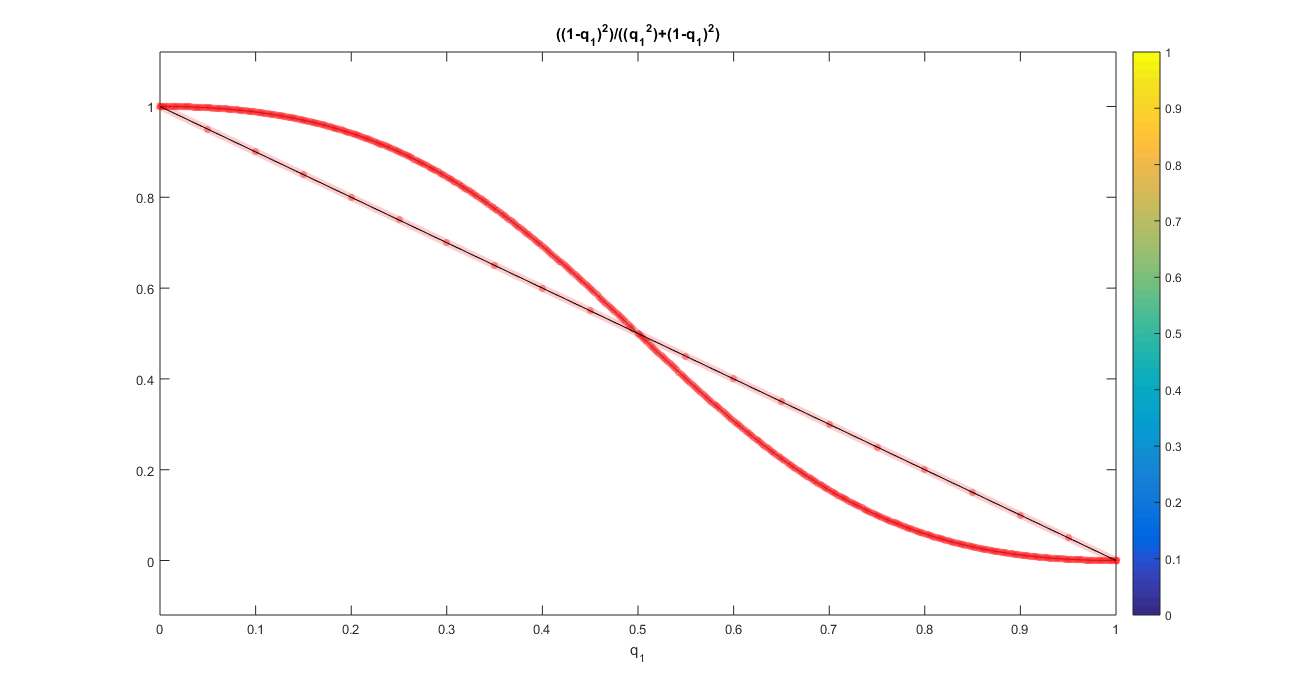
\includegraphics[width=90mm]{Error_2.png}
	\end{figure}


      %% Don't remove the empty line below.  Compilation will fail.
      
  \end{enumerate}
\end{enumerate}
